%
% ─── CAPITULO 8: VISUALIZACION DE FRACTALES 3D ──────────────────────────────────
%

En el capítulo \ref{chap:fractales-2D} introdujimos técnicas y código necesario para poder visualizar conjuntos de Julia y conjuntos de Mandelbrot 2-dimensionales en un canvas utilizando WebGL, todo ello apoyado en la teoría explicada en el capítulo \ref{chap:Julia-Mandelbrot}. Sin embargo, el objetivo de éste y de los tres capítulos anteriores es aplicar técnicas avanzadas de renderizado para poder visualizar fractales en tres dimensiones. Recordamos que explicamos en la introducción del capítulo \ref{chap:ray-tracing} que la mejor forma de renderizar fractales 3D es utilizando la técnica de `Ray Tracing', que en dicho capítulo explicamos con detalle. A pesar de ello y de conseguir escenas con varios objetos, materiales y movimientos de cámara no visualizamos nada lejanamente parecido a un fractal. Será en este capítulo en el que aprovecharemos toda la infraestructura y todo el código implementado hasta el momento en el `ray-tracer' del capítulo \ref{chap:ray-tracing} para graficar fractales tridimensionales.

Para ello, antes aún debemos asentar una serie de conceptos que son los que nos ayudarán a cumplir nuestro objetivo: el algoritmo \textit{Ray-Marching} y las conocidas como \textit{Signed Distance Functions} (SDFs). Con estos dos elementos combinados conseguiremos ver hermosas figuras fractales.

\section{El algoritmo Ray-Marching}
\label{section:ray-arching}

Hasta ahora siempre hemos calculado las intersecciones rayo-esfera de manera totalmente analítica, ya que es muy sencillo describir una esfera o un plano mediante una ecuación y solucionar esta ecuación en $t$, como vimos en las secciones \ref{subsection:esfera} y \ref{subsection:plano}. Sin embargo, no es tan sencillo encontrar ecuaciones que describan la superficie de los fractales. Es por esto que necesitamos otra manera de encontrar las intersecciones rayo-superficie. Aunque no tengamos una forma de calcular analíticamente la intersección, si contamos con funciones que nos estiman, fijado un punto, a qué distancia se halla este punto del fractal mediante una cota, las conocidas como SDFs. De igual manera, si fijamos un punto $p\in\R^3$, podemos calcular a qué distancia se encuentra dicho punto de una esfera o de un plano. 
% TODO Referenciar seccion de SDFs

El algoritmo \textit{Ray-Marching}, también conocido como \textit{Sphere-Tracing} es una técnica utilizada en Ray-Tracing y que se basa en estimar la distancia a la que se encuentra un punto de cada una de las superficies que componen la escena y avanzar en el rayo una distancia correspondiente a la mínima de estas distancias, pues se tiene la certeza de que al menos en una esfera de radio dicha distancia no hay ninguna intersección con ningún otro cuerpo. Una vez se ha avanzado en el rayo se repite esta operación y así sucesivamente hasta que la estimación de la distancia es lo suficientemente pequeña como para considerar que el punto interseca con la superficie.

Pongamos un ejemplo. Supongamos que tenemos una escena con una esfera tangente al plano horizontal $y=0$, un rayo $R$ fijo y queremos aplicar Ray-Marching para encontrar la intersección.

\begin{figure} [ht]
    \centering
    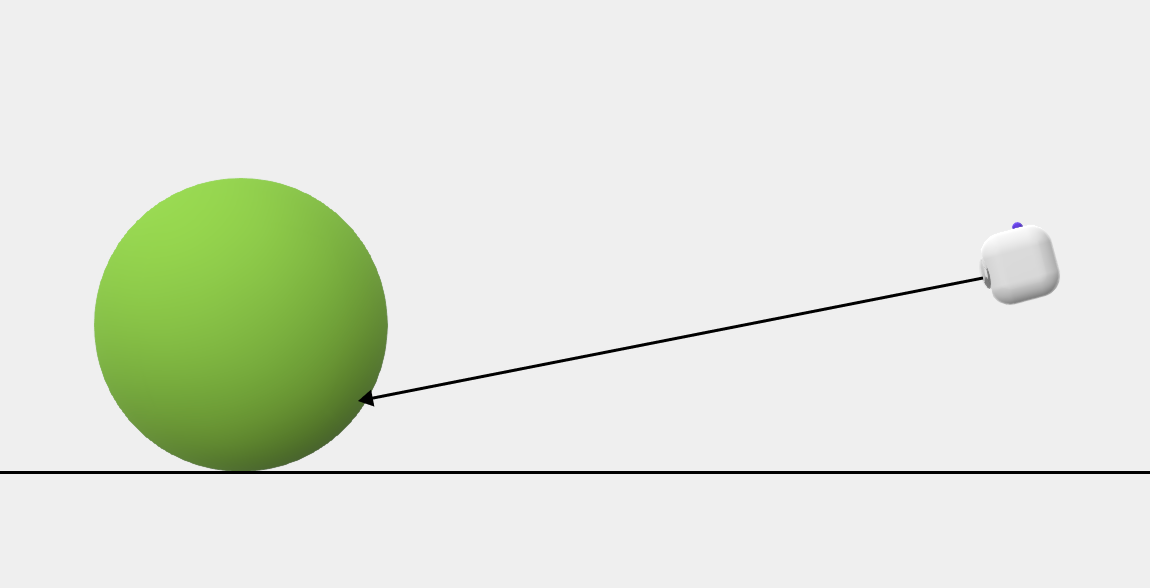
\includegraphics[scale = 0.2]{img/C8/situacion-inicial.png}
    \caption{Situación a la que aplicar Ray-Marching}
    \label{fig:RM-inicial}
\end{figure}

La distancia de un punto $p$ a una esfera $S$ de centro $c$ y radio $r$ es 
\begin{equation}
    \label{eq:distancia-punto-esfera}
    d(p,S) = \|p-c\| - r 
\end{equation}

y la distancia de un punto al plano $y=0$ es simplemente su componente $y$. Por tanto, partiendo del origen, calculamos la distancia a la esfera y la distancia al plano, vemos que es menor la distancia al plano, por lo que avanzamos en el rayo una distancia igual a la distancia que había al plano (imagen \ref{fig:iteraciones-RM} (a)). Seguidamente repetimos la operación: volvemos a calcular la distancia a la esfera y al plano. De nuevo es menor la distancia al plano, por lo que avanzamos en el rayo la misma distancia que había en el plano (imagen \ref{fig:iteraciones-RM} (b)).

\begin{figure}[ht]
    \centering
    \begin{tabular}{ccc}
      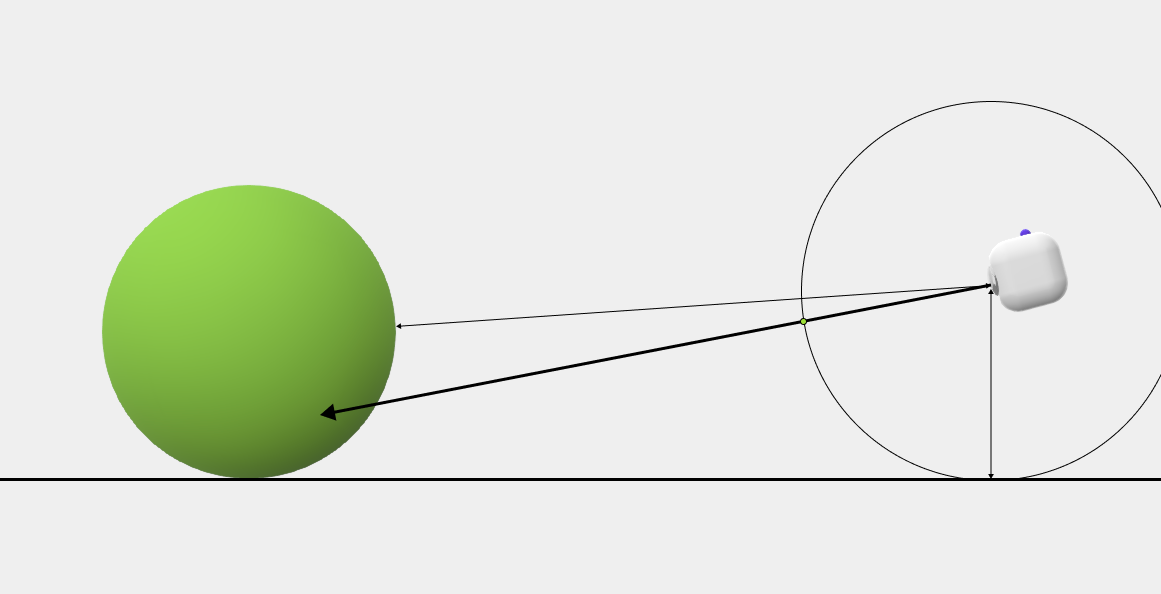
\includegraphics[scale=0.17]{img/C8/ray-marching-1.png} &     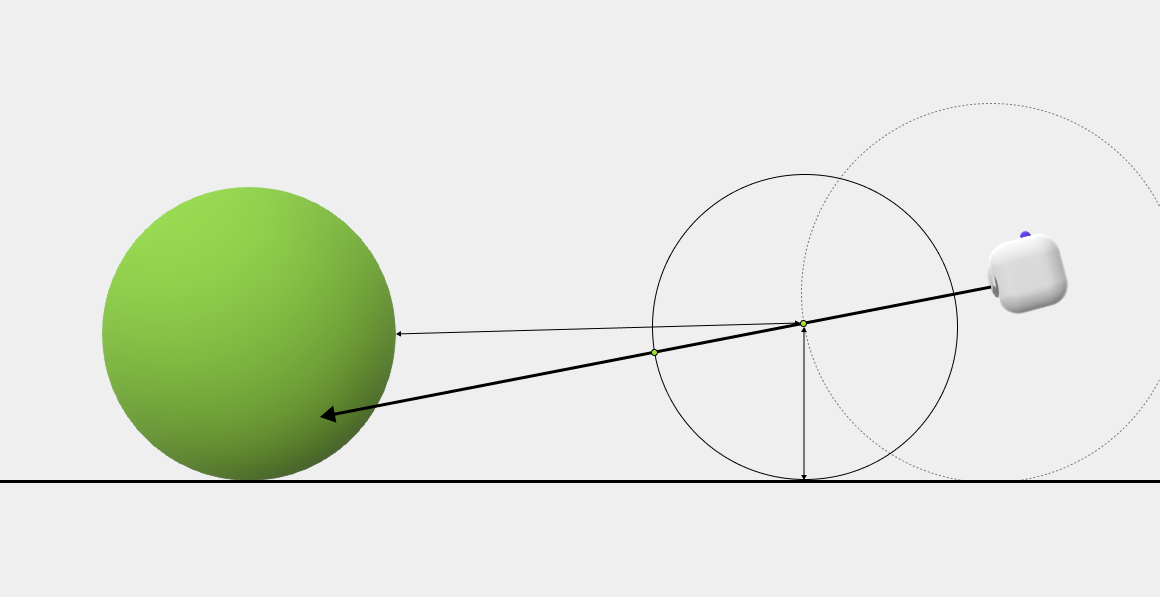
\includegraphics[scale=0.17]{img/C8/ray-marching-2.png} \\
    (a) Primera iteración & (b) Segunda iteración \\[6pt]
    \end{tabular}
    \caption{Dos primeras iteraciones de Ray Marching}
    \label{fig:iteraciones-RM}
\end{figure}

Si repetimos este proceso indefinidamente, llegará el momento en el que la distancia a la esfera será tan pequeña que consideraremos que el punto está en la esfera y habremos encontrado la intersección (imagen \ref{fig:finales} (a)). En caso de que no exista ninguna intersección, el algoritmo seguirá avanzando en el rayo, pero al no intersecar con ninguna superficie se avanzará indefinidamente (imagen \ref{fig:finales} (b)), por lo que hay que fijar una distancia máxima recorrida o un número máximo de iteraciones como parámetro del algoritmo.

\begin{figure}[ht]
    \centering
    \begin{tabular}{ccc}
      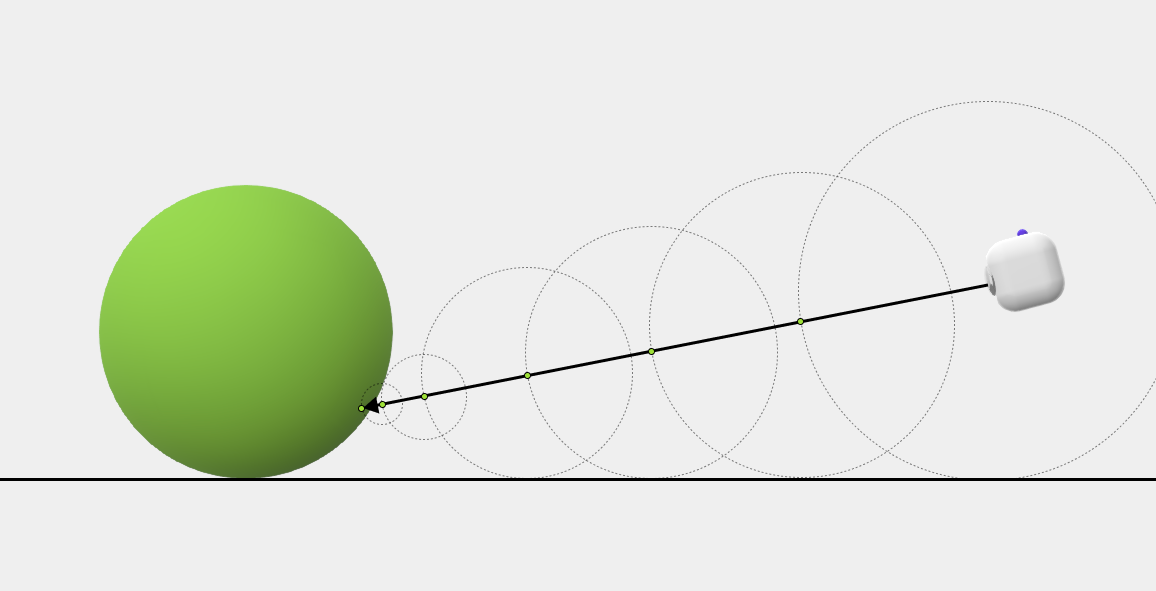
\includegraphics[scale=0.2]{img/C8/ray-marching-final.png} &     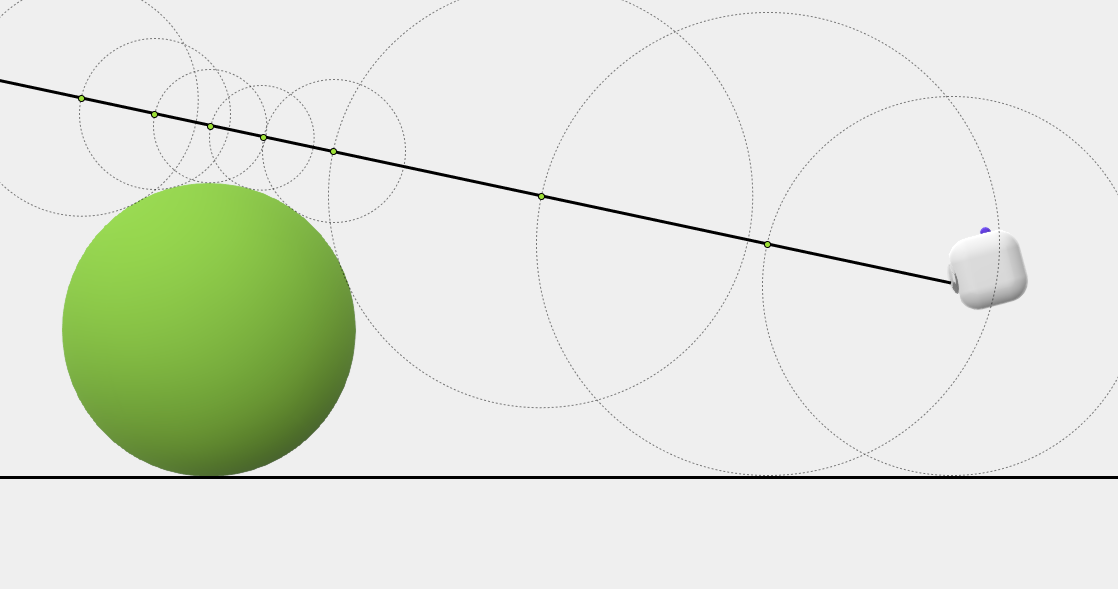
\includegraphics[scale=0.2]{img/C8/ray-marching-miss.png} \\
    (a) Encuentra intersección & (b) El rayo se pierde \\[6pt]
    \end{tabular}
    \caption{Posibles estados finales del algoritmo Ray-Marching}
    \label{fig:finales}
\end{figure}

Por tanto, el algoritmo, si consideramos un conjunto de $objetos$, un rato $R(t)=p_0 + \vec v t$ y un número máximo de avances en el rayo antes de decidir que no existe intersección $MAX\_STEPS$, se describiría como indica el algoritmo \ref{alg:Ray-Marching}.

\begin{algorithm}[H]
\caption{Ray-Marching} \label{alg:Ray-Marching}
%\KwData{Objects: Array de objetos, $\epsilon$: Distancia por debajo de la cual se considera intersección, R: Rayo $R(t)=p_0+\vec v t$}
\begin{algorithmic}
\State $p\gets lookfrom$
\State $steps \gets 0$

\While{$steps < MAX\_STEPS$} \Comment{También se puede fijar una distancia máxima}
    \State $min\_dist \gets MAX\_DIST$
    \State $i\gets 0$

    
    \While{$i < num\_objects$}\Comment{Cálculo de la mínima distancia}
        \State $dist \gets distancia(p, objects[i])$
        \If{$dist < min\_dist$}
            \State $min\_dist \gets dist$
            \State $index\gets i$
        \EndIf
        \State $i++$
    \EndWhile
    \If{$min\_dist < \varepsilon$}
        \State \textbf{Hay intersección} con $objects[index]$
    \Else
        \State $p\gets p + \vec v \cdot min\_dist$ \Comment{Avanzamos en el rayo}
    \EndIf
    \State $steps++$
\EndWhile
\State \textbf{No existe intersección}
\end{algorithmic}
\end{algorithm}

\begin{observacion}
\label{observacion:vector-normalizado}
    Cabe destacar un importante detalle, y es que a partir de este momento es indispensable que en la creación del rayo el vector dirección esté normalizado, pues si queremos avanzar $min\_dist$ unidades en la dirección $\vec v$ y $|v| \not= 1$ se avanzaría una distancia distinta y el algoritmo no funcionaría correctamente.
\end{observacion}

\subsection{Implementación de Ray-Marching en GLSL}

Veámos ahora cómo podemos llevarnos todos estos nuevos conocimientos a la GPU con GLSL. El objetivo ahora es modificar el fragment shader eliminando la dependencia de \verb|Hit_Sphere| y de \verb|Hit_Plane| para utilizar Ray-Marching para calcular las intersecciones. Realmente el resultado de estas modificaciones debería ser el mismo que en el final del capítulo anterior, pero ahora calcularemos las intersecciones de forma distinta. 

Lo primero que necesitaremos es una función que calcule la distancia de un punto a una esfera $S$. Esto es tan sencillo como implementar una función que calcule la fórmula \ref{eq:distancia-punto-esfera}.

\begin{lstlisting}
    
\end{lstlisting}